\chapter{马尔可夫链}

\section{随机过程}

随机过程研究的变量就是一个随机变量的序列$\{x_t|t\in T\}$,这个序列每一个元素都是随机变量,这里的$T$我们称为\textsl{参数集},我们常常把$t$看作是时间,$x(t)$为时刻$t$时的\textsl{状态},对于所有的$t\in T$,
$x(t)$的所有取值称为随机过程的\textsl{状态空间}。

对随机过程$\{x(t),t\in T\}$进行一次试验,其结果时$t$的函数,记为$X(t)$,称为随机过程的\textsl{样本函数}。

随机过程可以依照在任一时刻时连续型随机变量或者离散型随机变量,可以分为\textsl{离散随机过程}和\textsl{连续随机过程}。


\section{马尔可夫链}
\textsl{马尔可夫链}是一个特殊的随机过程,它的时间和状态都是离散的,并且马尔可夫链需要满足马尔可夫性质,也就是未来和过去是无关的
\begin{equation}
    P(x_{t+1}|x_1,x_2,\cdots,x_t)=P(x_{t+1}|x_t,x_{t-1},\cdots,x_{t-m})
\end{equation}

上面式子描述了一个$m$阶马尔可夫性质,当$m=0$时,就是所谓的\textsl{齐次马尔可夫}。
\begin{equation}
    P(x_{t+1}|x_1,x_2,\cdots,x_t)=P(x_{t+1}|x_{t})
\end{equation}

表述为概率图模型为

而$P(x_{t+1}|x_t)$这个概率用什么来表达呢?在马尔可夫链中定义\textbf{状态转移矩阵}
\begin{equation}
    [P_{ij}]_{N\times N},\ \ \ P_{ij}=P(x_{t+1}=j|x_t=i)
\end{equation}

\section{平稳分布}

所谓平稳分布,就是对于随机过程序列的每一个元素$x_i$,$x_i$在任意时刻服从的概率分布都是一样的,即
\begin{equation}
    P(x_1,\cdots,x_n)=P(x_{1+t},\cdots,x_{n+t})
\end{equation}

假设我们有如下马尔可夫链

\begin{figure}[H]
    \centering
    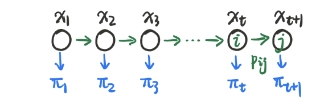
\includegraphics[scale=0.6]{figures/马尔可夫链.png}
    \caption{马尔可夫链}
\end{figure}

它在$t+1$时刻的概率分布表达为
\begin{equation}
    \pi_{t+1}(x^*)=\int \pi_t(x)\cdot P(x\rightarrow x^*)dx
\end{equation}

通俗来讲,它实际上就是所有可能转移的状态$x_{t+1}$的概率分布的和,那么什么随机分布呢?

假如这里存在一个$pi$,这里的$pi$和前面的$\pi_t$和$\pi_{t+1}$一点儿关系没有,假如$\pi$是一个概率分布,那么就可以被写成无限维向量的形式
\begin{equation}
    \pi=[\pi(1),\pi(2),\cdots,\pi(t),\cdots], \ \ \ \sum_{i=1}^{\infty}\pi(i)=1
\end{equation}

使得
\begin{equation}
    \pi(x^*)=\int \pi(x)\cdot P(x\rightarrow x^*)dx
\end{equation}

我们就称$\{\pi(k)\}$是马尔可夫链的平稳分布,即每个时刻都符合同一个概率分布$\pi$。

下一个问题是,什么样的分布可以称为平稳分布,也就是我们怎样才能构建出一个马氏链让他收敛到一个平稳分布当中呢?
这里我们引入一个条件,就是\textsl{Detailed Balance}:
\begin{eqnarray}
    \pi(x)\cdot P(x\rightarrow x^*)=\pi(x^*)\cdot P(x^*\rightarrow x)
\end{eqnarray}

这个式子表明任意两个状态之间,使用概率分布作为转移概率的结果都是可逆的,那么这两个状态之间的分布肯定都是一样的。满足\textsl{Detailed Balance}一定是平稳分布
\begin{equation}
    \begin{aligned}
        \int \pi(x)\cdot P(x\rightarrow x^*)dx&=\int \pi(x^*)\cdot P(x^*\rightarrow x)dx\\
        &=\pi(x^*)\int P(x^*\rightarrow x)dx
        &=    \pi(x^*)
    \end{aligned}
\end{equation}

